\setchapterimage[2cm]{../images/header-sunflowers.png}
%\setchapterpreamble[u]{\margintoc}
\chapter{Characterization of the sunflower molecules}
\labch{sunflowers}

\section{Sunflower design}

\begin{marginfigure}
    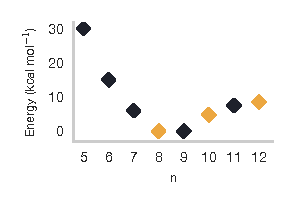
\includegraphics{sulflower-strain}
    \caption[Strain of thiophenic circulenes]{Strain of thiophenic circulenes with n rings}
    \labfig{sulflower-strain}
\end{marginfigure}

To start designing a family of molecules, first we must clearly state their defining pattern.
For this purpose, we adopt Chernichenko et al.'s own proposal: \q{a novel class of heterolytic circulenes}.
We start expanding the model by answering the question: are thiophene based circulenes with other than 8 rings stable enough to be worth considering?
The answer is in the original paper itself.
\reffig{sulflower-strain}, which was recreated to use our calculation level and adapt to the style of the document, shows that 8 ring structures are the most stable alongside 9 ring ones.
The details about this calculation are further explained in \refsec{study-of-stability}.
However, considering their low relative energies and the fact that they would have an even number of electrons even if (which would greatly simplify later calculations), 10 and 12 ring sunflowers were also chosen as part of the study.

Expanding upon this idea to allow for further heteroatom substitution, we ended up with the templates in \reffig{sunflower-skeletons}.
The possibilities were numerous, but we settled for S, Se, As and P substitutions on X$_1$ sites, and N substitutions in some cases in X$_2$ sites.
A full table detailing all of the structures that were generated and will comprise this study can be found in \reftab{sunflower-family}, as well as the short names or IDs that were given to each species based on its composition and number of petals for the sake of abbreviation.

\begin{figure*}
    \centering
    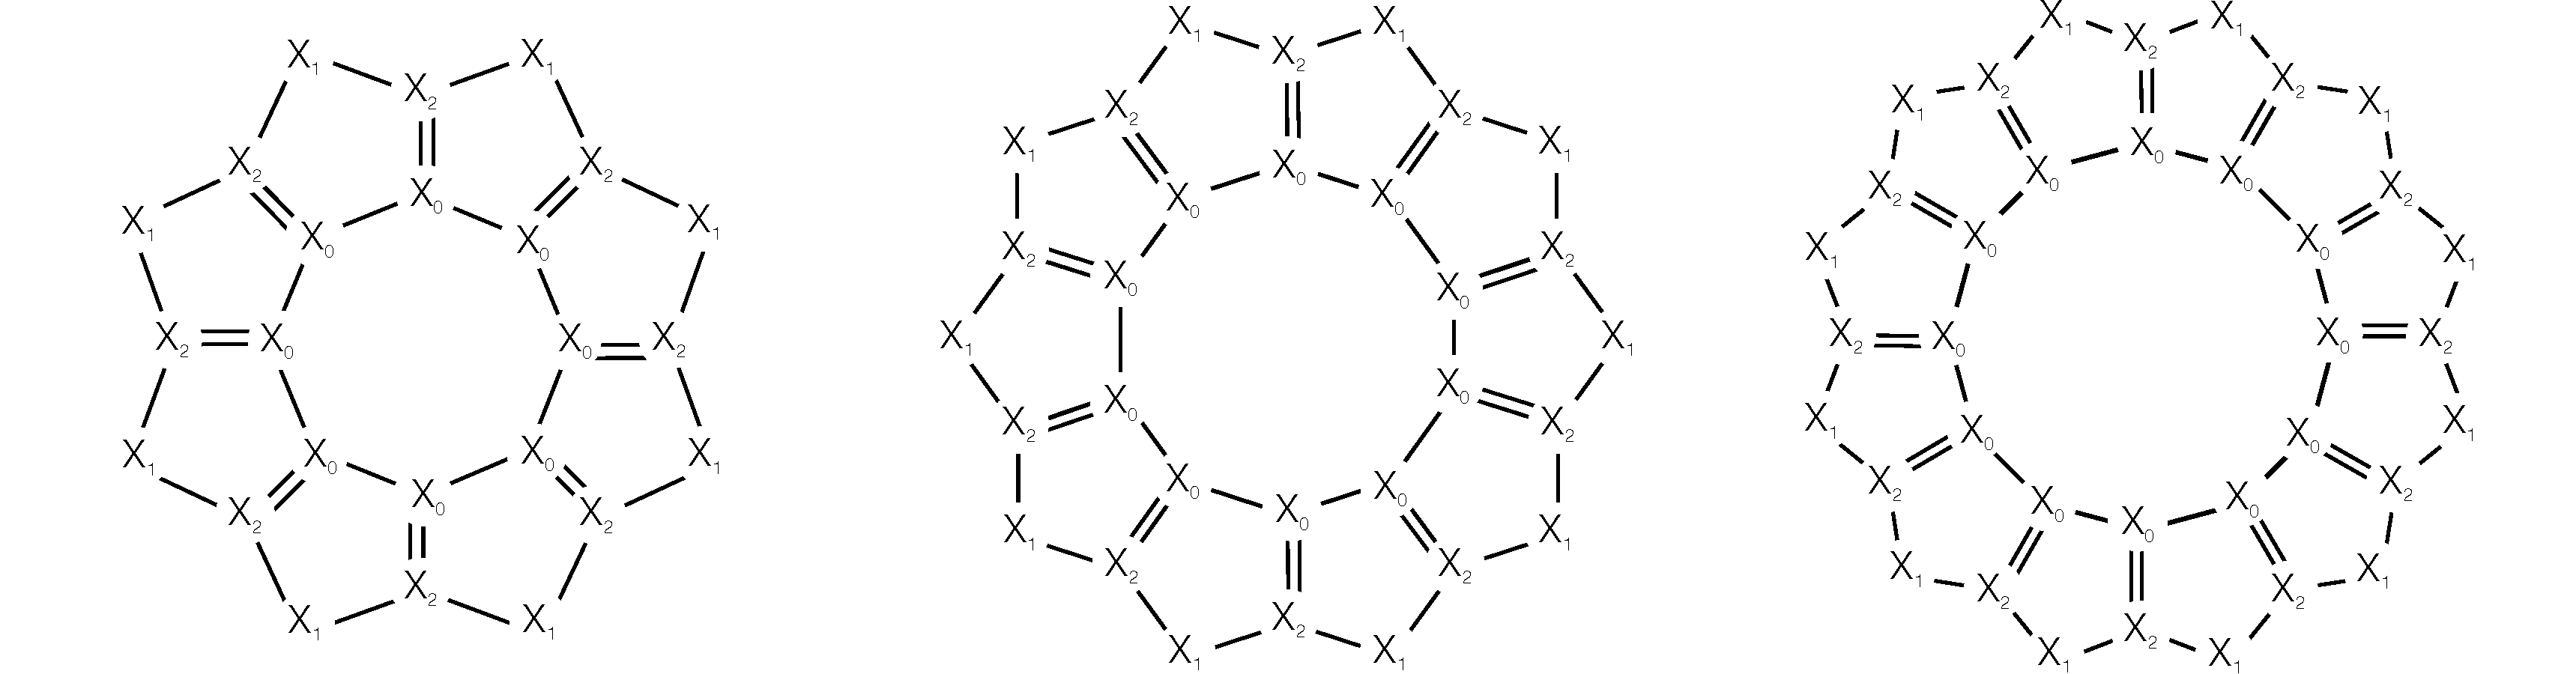
\includegraphics{sunflower-skeletons}
    \caption[General structures of the sunflower family]{From left to right, general structures of the 8, 10 and 12 ring sunflowers}
    \labfig{sunflower-skeletons}
\end{figure*}

\begin{table}
    \centering
    \caption[Sunflowers in this study]{Subset of the sunflower family that is going to be studied}
    \begin{tabular}{@{}cccrrr@{}}
        \toprule
        &&& \multicolumn{3}{c}{number of rings} \\
        X$_0$ & X$_1$ & X$_2$ & \multicolumn{1}{c}{8} & \multicolumn{1}{c}{10} & \multicolumn{1}{c}{12} \\
        \midrule
        C & S & C & S08 & S10 & S12 \\
        C & Se & C & Se08 & Se10 & Se12 \\
        C & As & C & As08 & As10 & As12 \\
        C & As & N & AsN08 & AsN10 & AsN12 \\
        C & P & C & P08 & P10 & P12 \\
        C & P & N & PN08 & PN10 & PN12 \\
        \bottomrule
    \end{tabular}
    \labtab{sunflower-family}
\end{table}


\section{Study of geometry}
\labsec{study-of-geometry}

\begin{marginfigure}
    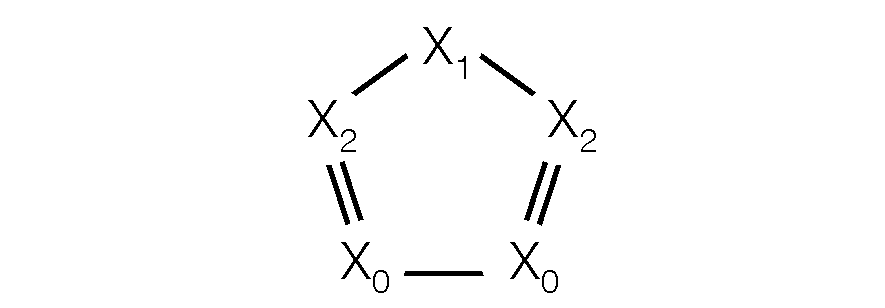
\includegraphics{pentagon-structure}
    \caption[Thiophene-like structure template]{Thiophene-like structure template (hydrogen is added to adjust for neutrality as needed)}
    \labfig{pentagon-structure}
\end{marginfigure}

Coordinate files for all of the designed sunflowers were created using 3D molecule modeling software.
Then, they were optimized at the M06-2X/def2SVP calculation level.

\begin{figure}
    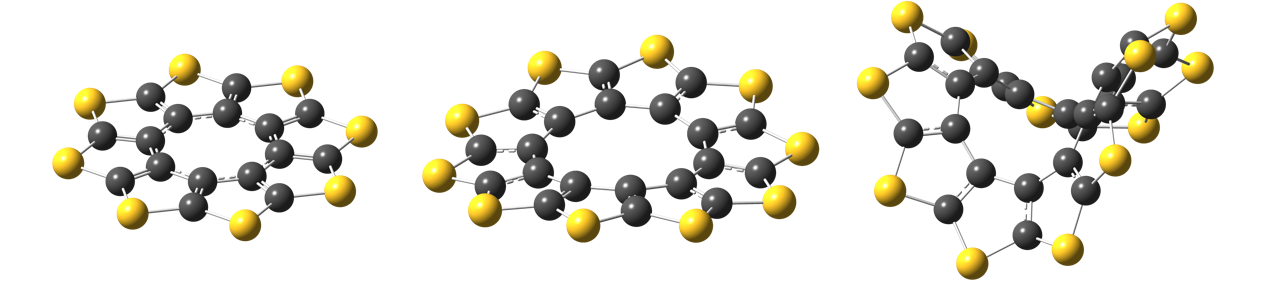
\includegraphics{sunflower-shapes}
    \caption[Shape of the sunflowers]{Shape of optimized S08, S10 and S12, from left to right (note the progressive increase in their deviation from planarity)}
    \labfig{sunflower-shapes}
\end{figure}

Using the output files for these calculations, all of the bond distances in all of the systems were extracted using Python.
Then, the bonds were grouped by type: inner (I, bonds between X$_0$ atoms, which were carbon in all cases), middle (M, between X$_0$ and X$_2$ atoms, which were either C-C or C-N bonds), and outer (O, between X$_2$ and X$_1$ atoms).
The mean and standard deviation of these groups were computed for all of the flowers.
Additionally, thiophene-like pentagonal structures of the form displayed in \reffig{pentagon-structure} were modeled and optimized, and their bond length data was compared with the rest and presented in \reftab{bond-length-study}.

How is this information useful?
In the first place, it allows us to easily compare the average length of each bond type as the number of units increases.
More interestingly, it serves as a way to assess the nature of each bond group.
Take the inner C-C bonds.
In all cases, the average length lies between the usual values for single and double C-C bonds,\sidenote{\SI{1.54}{\angstrom} for single and \SI{1.34}{\angstrom} for double bonds \fix{add reference}} an information that immediately suggests us that the flowers might be conjugated systems with $\pi$ electron delocalization.
However, it could also be possible that there were equal amounts of single and double bonds, and that these apparently conjugated bond lengths were just a the result of a lousy statistical approximation.
That's why the $\sigma$ metric was also computed.
Groups with a relatively high $\sigma$ such as the I bonds of As08, As12, P08 and P12 are actually composed of longer and shorter bonds, and it's likely that their $\pi$ electrons aren't delocalized.
On the other hand, groups with small $\sigma$ values are more likely to correspond to conjugated systems, which may be stabilized by electron delocalization.
This concept of bond length equalization and conjugation may be tied to that of aromaticity, where equalized C-C bonds could be a sign of it, and uneven ones could indicate non aromaticity or antiaromaticity.\sidecite{zhongfang05} This topic will be covered in greater detail in \refsec{study-of-aromaticity}.

\begin{table}
    \centering
    \caption[Bond length study]{Bond length statistics for each studied species, units are \si{\angstrom}, and $\tilde{x}$ and $\sigma$ are the mean and the standard deviation}
    \begin{tabular}{@{}rlcccccc@{}}
        \toprule
        && \multicolumn{2}{c}{I (X$_0$-X$_0$)} & \multicolumn{2}{c}{M (X$_0$-X$_2$)} & \multicolumn{2}{c}{O (X$_1$-X$_2$)} \\
        && $\tilde{x}$ & $\sigma$ & $\tilde{x}$ & $\sigma$ & $\tilde{x}$ & $\sigma$ \\
        \midrule
        \multirow{4}{*}{S} & ring & 1.429 & - & 1.367 & 0.000 & 1.719 & 0.000 \\
        & 08 & 1.423 & 0.000 & 1.377 & 0.000 & 1.754 & 0.000 \\
        & 10 & 1.482 & 0.000 & 1.399 & 0.000 & 1.712 & 0.000 \\
        & 12 & 1.466 & 0.004 & 1.389 & 0.000 & 1.732 & 0.004 \\
        \\
        \multirow{4}{*}{Se} & ring & 1.434 & - & 1.363 & 0.000 & 1.857 & 0.000 \\
        & 08 & 1.454 & 0.000 & 1.385 & 0.000 & 1.865 & 0.000 \\
        & 10 & 1.478 & 0.003 & 1.389 & 0.000 & 1.861 & 0.004 \\
        & 12 & 1.466 & 0.007 & 1.381 & 0.000 & 1.877 & 0.005 \\
        \\
        \multirow{4}{*}{As} & ring & 1.468 & - & 1.354 & 0.000 & 1.918 & 0.000 \\
        & 08 & 1.434 & 0.050 & 1.448 & 0.000 & 1.859 & 0.008 \\
        & 10 & 1.436 & 0.000 & 1.454 & 0.001 & 1.856 & 0.001 \\
        & 12 & 1.435 & 0.042 & 1.446 & 0.002 & 1.867 & 0.007 \\
        \\
        \multirow{4}{*}{AsN} & ring & 1.495 & - & 1.283 & 0.000 & 1.854 & 0.000 \\
        & 08 & 1.434 & 0.000 & 1.361 & 0.000 & 1.858 & 0.000 \\
        & 10 & 1.450 & 0.001 & 1.364 & 0.001 & 1.856 & 0.004 \\
        & 12 & 1.440 & 0.004 & 1.357 & 0.001 & 1.873 & 0.006 \\
        \\
        \multirow{4}{*}{P} & ring & 1.467 & - & 1.359 & 0.000 & 1.794 & 0.001 \\
        & 08 & 1.410 & 0.048 & 1.445 & 0.000 & 1.764 & 0.006 \\
        & 10 & 1.431 & 0.000 & 1.471 & 0.000 & 1.736 & 0.000 \\
        & 12 & 1.429 & 0.045 & 1.462 & 0.002 & 1.747 & 0.005 \\
        \\
        \multirow{4}{*}{PN} & ring & 1.485 & - & 1.293 & 0.000 & 1.707 & 0.000 \\
        & 08 & 1.404 & 0.000 & 1.364 & 0.000 & 1.752 & 0.000 \\
        & 10 & 1.448 & 0.000 & 1.385 & 0.000 & 1.715 & 0.001 \\
        & 12 & 1.435 & 0.002 & 1.378 & 0.001 & 1.732 & 0.004 \\
        \bottomrule
    \end{tabular}
    \labtab{bond-length-study}
\end{table}


\section{Study of stability}
\labsec{study-of-stability}

Using the output files from the previous step, specifically those from the initial optimization, calculations related to the energies of the flowers were performed in order to assess their stabilities.

\subsection{Ring strain}
\labsec{ring-strain}
Ring strain may be defined as a kind of instability that arises when angles of the bonds in a cyclic molecule deviate from their optimal values, which they would be able to adopt if they weren't coiled in the shape of a ring.
The energy associated to this phenomenon can serve as a way to compare the stabilities of flowers with different numbers of petals, as it was done in the original paper and reproduced in \reffig{sulflower-strain}.
Its calculation relies on the design of an homodesmotic reaction.
What does this mean?
In a homodesmotic reaction, the number of atoms and the type of hybridations in the products are the same as in the reactants.
Our goal is to devise a chemical equation where the strained structure appears in only one of its sides and the rest of the chosen molecules don't present any strain effects.\sidecite{vidalvidal18}
If we manage to create such an equation, the reaction energy will correspond to the strain, as the rest of the components of the energy should nullify themselves between the two sides of the reaction.

In this case, apart from the sunflower structure B, the equations that were designed included molecules A and C, non-cyclic structures composed of 3 and 2 petals. \marginnote{
	\begin{equation}
        \labeq{homodesmotic-equation}
        E_\text{strain} = \frac{E_B + nE_C - nE_A}{n}
	\end{equation}
} By following this reaction, which is fully displayed in \reffig{homodesmotic}, the strain energy was calculated as shown in \refeq{homodesmotic-equation}.

\begin{figure}
    \centering
    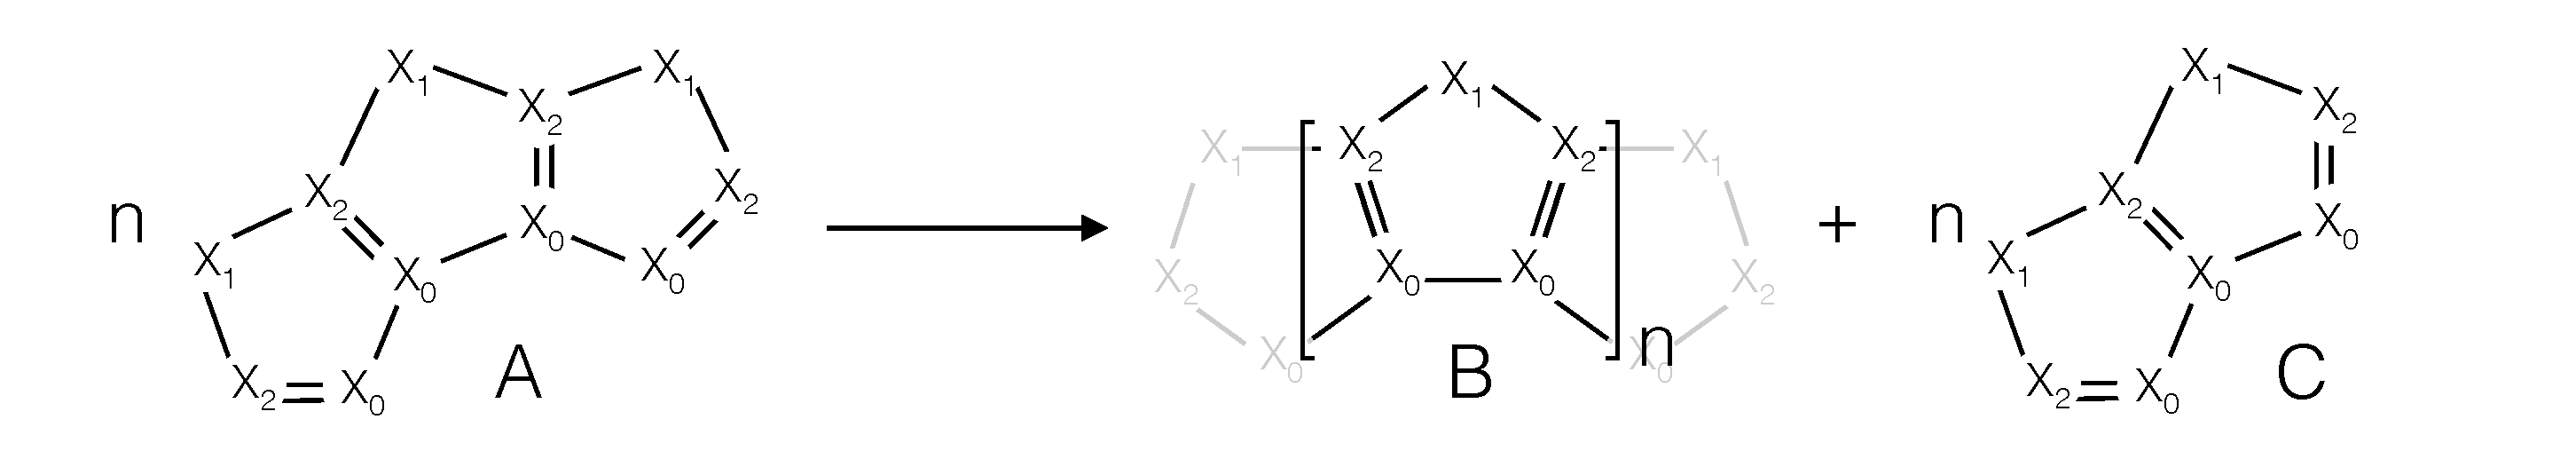
\includegraphics{homodesmotic}
    \caption[Homodesmotic reaction used to calculate strain energies]{Homodesmotic reaction used to calculate strain energies}
    \labfig{homodesmotic}
\end{figure}

This calculation, which is the one that was used to generate the previous sulflower stability curve \reffig{sulflower-strain}, was applied to all of the sunflowers of the study, and the resulting strain energies are presented in \reffig{sunflower-stability}.
As it can be seen, the strain energies always increase with the number of petals (as it's the case for the original sulflower series).
However, it may be noted that their increase follows slightly different tendencies.
Notable examples are the P family, where the 8 and 10 petal species have very similar strains; and the Se, As and AsN families, where the energies of the 10 and 12 petal structures are very close.
These energy values are an useful indication of the relative strains of the different species within a family, and an estimation of their
stabilities with respect to the original sulflower.
Nevertheless, it should be kept in mind that this calculation is an approximation, and that the values of the so called strain energy might be accounting for other effects such as conjugation stabilization or repulsion between the heteroatoms.

\begin{figure}
    \centering
    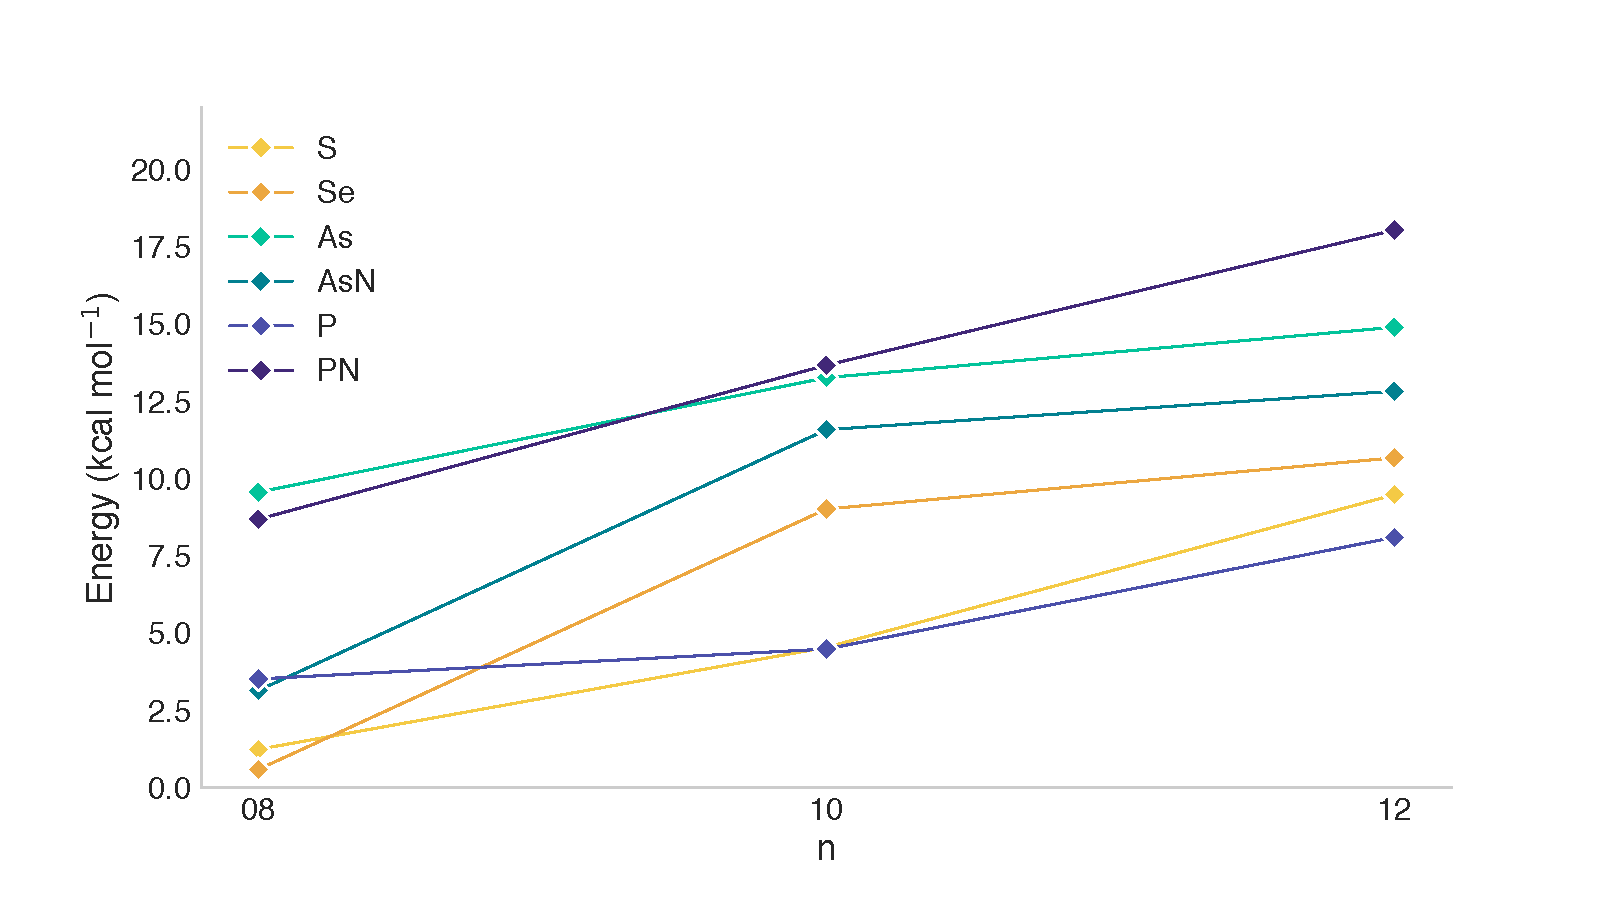
\includegraphics{sunflower-stability}
    \caption[Strain energies of sunflower groups]{Strain energies of all of the studied sunflower groups}
    \labfig{sunflower-stability}
\end{figure}


\section{Study of aromaticity}
\labsec{study-of-aromaticity}

Aromaticity is a property related to molecules that contain a ring or a chain of resonance bonds that increases their stability.
It’s typically found in flat ring structures, although the definition has been discussed and expanded since its initial association to benzene\sidecite{faraday1825} and there are other varieties such as annulenic, azulenic, inorganic, homoaromatic, three-dimensional, $\sigma$-electron, and even metallic electron aromaticity.\sidecite{zhongfang05}
Considering their ringed structure and possibly high conjugation, we wondered if the sunflowers could present any kind of aromatic tendencies.
Having already studied their degree of bond length equalization in \refsec{study-of-geometry}, we set out to assess their aromaticity from the point of view of their magnetic properties.

\subsection{Nucleus-independent chemical shift}
\labsec{nics}
Since its introduction in 1996 by Schleyer et al.\sidecite{schleyer96}, Nucleus-independent chemical shift (NICS) has become the most popular and widely used technique to estimate aromaticity in a quantitative way.
It's based on the study of electronic ring currents.
As the electrons in the possibly-aromatic systems have a certain degree of free circulation, an external magnetic field perpendicular to the main plane of the system is able to induce a ring current.
Said ring currents generate their own magnetic field, which can weaken or strengthen the effect of the external field, resulting in decreased or increased NMR chemical shifts.
Aromatic systems will experience shielding on the inside of the ring and deshielding on the outside.
Antiaromatic systems will experience the opposite.

\subsubsection{The basic application of NICS}
NICS is usually applied to single rings, and quantified by computing the absolute magnetic shielding at key locations.
This key location is usually one of the following: the center of the ring (calculated as the non-weighted mean of the positions of the heavy atoms), several points along a central axis perpendicular to the plane of the ring (calculated trivially in planar rings as the plane that passes through any three ring atoms), at several points on a grid perpendicular to the plane of the ring, or as three dimensional isosurfaces using dense grids.

\subsubsection{A custom solution for non-planar molecules}

\begin{marginfigure}
    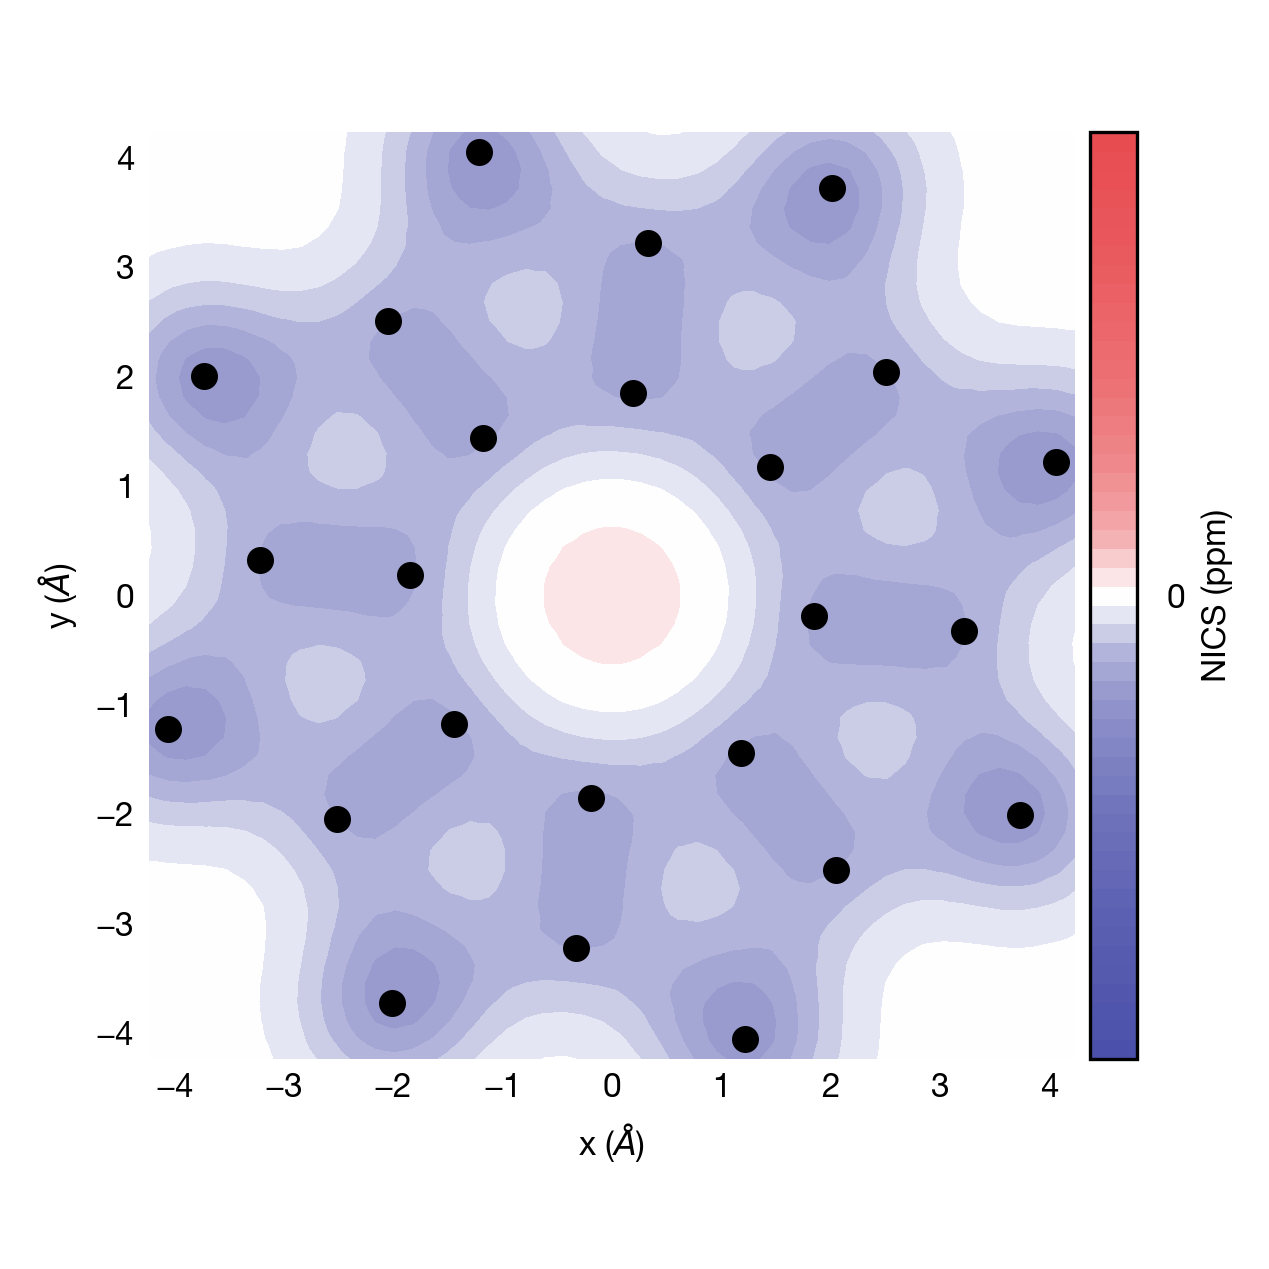
\includegraphics{s08-2d}
    \caption[NICS applied to sulflower]{Custom NICS technique applied to the original 8 petal sulflower molecule as a sample of the legacy approach}
    \labfig{s08-2d}
\end{marginfigure}

A seen in \reffig{sunflower-shapes} in \refsec{study-of-geometry}, 8 petal sunflowers are perfectly planar.
In previous studies, NICS calculations on flat grids parallel to their planes were applied with success.
All of the points of the grid were equidistant to the plane of the molecule to be able to properly compare their values (the magnitude of the magnetic shielding decreases the farther away from the molecule that it is measured).
The positive values of the magnetic shielding were plotted in red and the negative ones in blue, which overlaid over the atoms of the flower, resulted in graphs like \reffig{s08-2d}.
However, 10 and 12 petal sunflowers have bended and warped shapes, and the \q{general plane} of the molecule is no longer a plane.
In order to translate the old method, a new approach was developed and applied.
The idea of extending a grid of points over the surface of the system and plotting it as a 2D projection is maintained, but what is exactly the surface of a non planar molecule, and how can it be generalized for non planar molecules?

Defining the concept of \q{general surface} for a warped ring is a tricky task, but we've set on the following description: a 3D surface that is equidistant to all of the heavy atoms of a molecule and to all of the middle points of their bonds, and that follows a smooth and intuitive tendency in the places where are neither atoms nor bonds. A general surface could be loosely thought of as a blanket that was being draped over a physical molecular model of the system, sitting on the places where there are balls and sticks, and covering the empty spaces smoothly without caving in.

To mathematically model such an idea, several approaches were evaluated and tested,\sidenote{Such as using interpolation algorithms to calculate the grid points in the empty spaces, or generating compound surfaces by tiling all of the possible planes based on groups of three atoms.} but in the end, the method was based on linearly combining a set of simple 3D cartesian functions.

This idea was born while thinking about the curvature of the largest sunflowers.
\q{This Se10 molecule looks like it has the shape of a saddle.\sidenote{The equation of a basic saddle is essentially $z=x^2-y^2$.} What if we could find the precise parameters for a saddle that adjusted to the shape of this molecule?}
This concept was expanded to include a wider variety of molecules and shapes: there's a limit to the angles and deformations that a ring in a molecule can display... so therefore, it should be possible to get a decent approximation to any molecular surfaces by combining and fine tuning a selection of common 3D shapes in the form of functions.
The remaining question is... how can we find which 3D functions should be used, and what coefficients should be assigned to them?
The functions were picked out by hand, and will later be enumerated and justified.
The coefficients, however, had to be calculated somehow.
Our solution, which will be fully explained hereunder, relies upon the core concepts of statistical learning.

\begin{margintable}
    \centering
    \caption[xyz coordinates]{xyz coordinates of the atoms of Se10}
    \begin{tabular}{@{}S[table-format=1.4]
                       S[table-format=1.4]
                       S[table-format=1.4]@{}}
        \toprule
        $x$ & $y$ & $z$ \\
        \midrule
        0.9154 & 0.0917 & 0.0236 \\
        -0.0971 & 0.9542 & 1.9687 \\
        1.0978 & 0.8552 & 1.2691 \\
        1.8126 & 1.7897 & 3.3270 \\
        \multicolumn{3}{c}{{\ldots}}
    \end{tabular}
    \labtab{xyz}
\end{margintable}

First off, we start with just the coordinate file of the optimized structure of the studied molecule.
We will use Se10 as an example.
This file should contain the position of each of the atoms in the 3D cartesian space relative to the origin of coordinates (i.e., an xyz file).
In order to stabilize the calculations and apply the method properly, the molecule has to undergo two transformations: it has to be translated so that its center coincides with the origin of coordinates $(0,0,0)$; and it has to be rotated so that its main axis aligns with $z$, or $(0,0,1)$.

The first one is trivial, the centroid of the ring is calculated as the mean of all of the positions of the atoms, and is then subtracted from them.

The second one, the rotation, is not as straightforward.
First, the main axis of the molecule has to be calculated.
In this case, the main axis is defined as the direction where there is the least amount of variance.
Mathematically, it's equal to the eigenvector that corresponds to the smallest eigenvalue of the covariance matrix of the relative coordinates.\sidenote{That is, the coordinates after having been translated to $(0,0,0)$ in the previous step}
After having calculated such a vector, it's a matter of calculating the angle that it forms with the $z$ axis using simple dot product, and designing and applying an adequate rotation matrix.

Se10, as well as all of the other sunflowers of the study, only contains heavy atoms that are relevant to the problem, so we can just ignore their chemical elements and treat every point equally.
However, it should be noted that in other cases there might be irrelevant atoms such as hydrogens, or parts of the molecule that don't belong to the surface that we are trying to identify.
In those situations, special care should be taken: the transformation operations have to be designed around the important atoms, but they should be applied to the whole system.

At this point, the relevant part of the molecule (i.e. the ring object of study), should be centered and aligned with the $z$ axis.
All of these preparatory steps ensure the optimal application of the actual method.

The method itself consists in the optimization of the coefficients of a multiple linear regression model.\marginnote{
	\begin{equation}
        \labeq{multiple-linear-regression}
        f_i \approx \beta_0 + \beta_1 x_{i1} + \beta_2 x_{i2} + ... + \beta_p x_{ip} \quad i=1,...,n
	\end{equation}
} %
A linear regression model with $p$ predictors and $n$ data points, as shown in \refeq{multiple-linear-regression}, consists of several elements.
$y$ is the target feature, the one that we wish to predict.
The various $x$ are the predictors, variables on which we base our predictions.
The various $\beta$ values are the coefficients that accompany the predictors and that we want to approximate.

In our case in particular, the bits of real data that we have -our ground truth- are the coordinates of the atoms of the molecule, which include $x$, $y$ and $z$ values.
Looking at it from the point of view of statistical learning, the problem could be defined as \q{designing a model that predicts the values of $z$ by using the values of $x$ and $y$}.
If such a model was developed, we could just input a square grid of $(x,y)$ values and get the height (or $z$ value) that they should be placed at to conform to our concept of general surface.
There is just a problem with this approach: using just $x$ and $y$ by themselves as the predictors is not enough to generate the kind of warped, wavy surfaces that we're looking for!
Just by adding different proportions of $x$ and $y$, the best one that we could get would be a tilted plane.%
\begin{margintable}
    \centering
    \caption[Calculated predictors]{Calculated predictors, with $f=\sqrt{(x^2+y^2)}$}
    \begin{tabular}{@{}S[table-format=1.4]
                       S[table-format=1.4]
                       S[table-format=1.4]
                       S[table-format=1.4]@{}}
        \toprule
        {$x^2$} & {$y^2$} & {$xy$} & {$f$} \\
        \midrule
        0.0230 & 1.8121 & 1.7809 & 3.3327 \\
        1.9680 & 0.9151 & 0.0901 & 0.3023 \\
        1.2690 & 0.0971 & 0.9504 & 1.3968 \\
        3.3270 & 1.0971 & 0.8505 & 1.3269 \\
        \multicolumn{4}{c}{{\ldots}}
    \end{tabular}
    \labtab{all-predictors}
\end{margintable}%
That is where the 3D surface selection approach gets mixed in.
We can combine the $x$ and $y$ values in certain ways in order to generate a wider variety of basic shapes to linearly combine, resulting in a better set of predictors.
For this problem, the following set of predictors was chosen: $x^2$ and $y^2$ (half cylinders, which result in a saddle when subtracted and a dome when added), $xy$ (a saddle aligned with the diagonal $x=y$), and $\sqrt{(x^2+y^2)}$ (a cone).\sidenote[][*9]{It should be noted that this is not proper statistical learning practice: in a real application the predictors shouldn't have any correlation between them.}

Having defined the elements of the model, its a matter of transforming the $x$ and $y$ values into their function forms, initializing a linear model, training it with these predictors and the values of the target variable $z$, and retrieving the coefficients.
This is all done using the convenient scikit-learn module,\sidecite{scikit-learn} a machine learning framework for the Python language.
Without delving deep deep in their lineal model's inner workings, it can be said that it relies on two key parts: a cost function that measures its deviation from the target, and an algorithm that minimizes it by iteratively modifying its coefficients.
When the model has been trained, its accuracy is measured by computing the values of the $R^2$ metric for two sets of points: the original coordinates of the atoms (i.e., the data points that the model is based on), and the middle points of each of the bonds (i.e. a collection of new data that the model hadn't previously known about).

All of this operations have been combined and encapsulated inside a custom Python command line application available in the author's GitHub account\sidecite{github-nics}.

Continuing with the running example, the output of the adjustment of Se10 would be as follows.
\begin{lstlisting}[label=se10-output, style=kaolstplain]
$ python nics.py surface se10.xyz

    Linear regression results:
                     x^2: -0.1056911
                     y^2:  0.1064271
                      xy:  0.1375246
         sqrt(x^2 + y^2): -0.0081293

    R2 score: 0.978916
    R2 score of atom midpoints: 0.988095
\end{lstlisting}

As a way of clearly displaying the result, the idea behind the method, and the elements of the linear combination, the functions have been plotted individually (omitting the last one due to its low contribution) in \reffig{linear-combination}.

\begin{figure*}
    \centering
    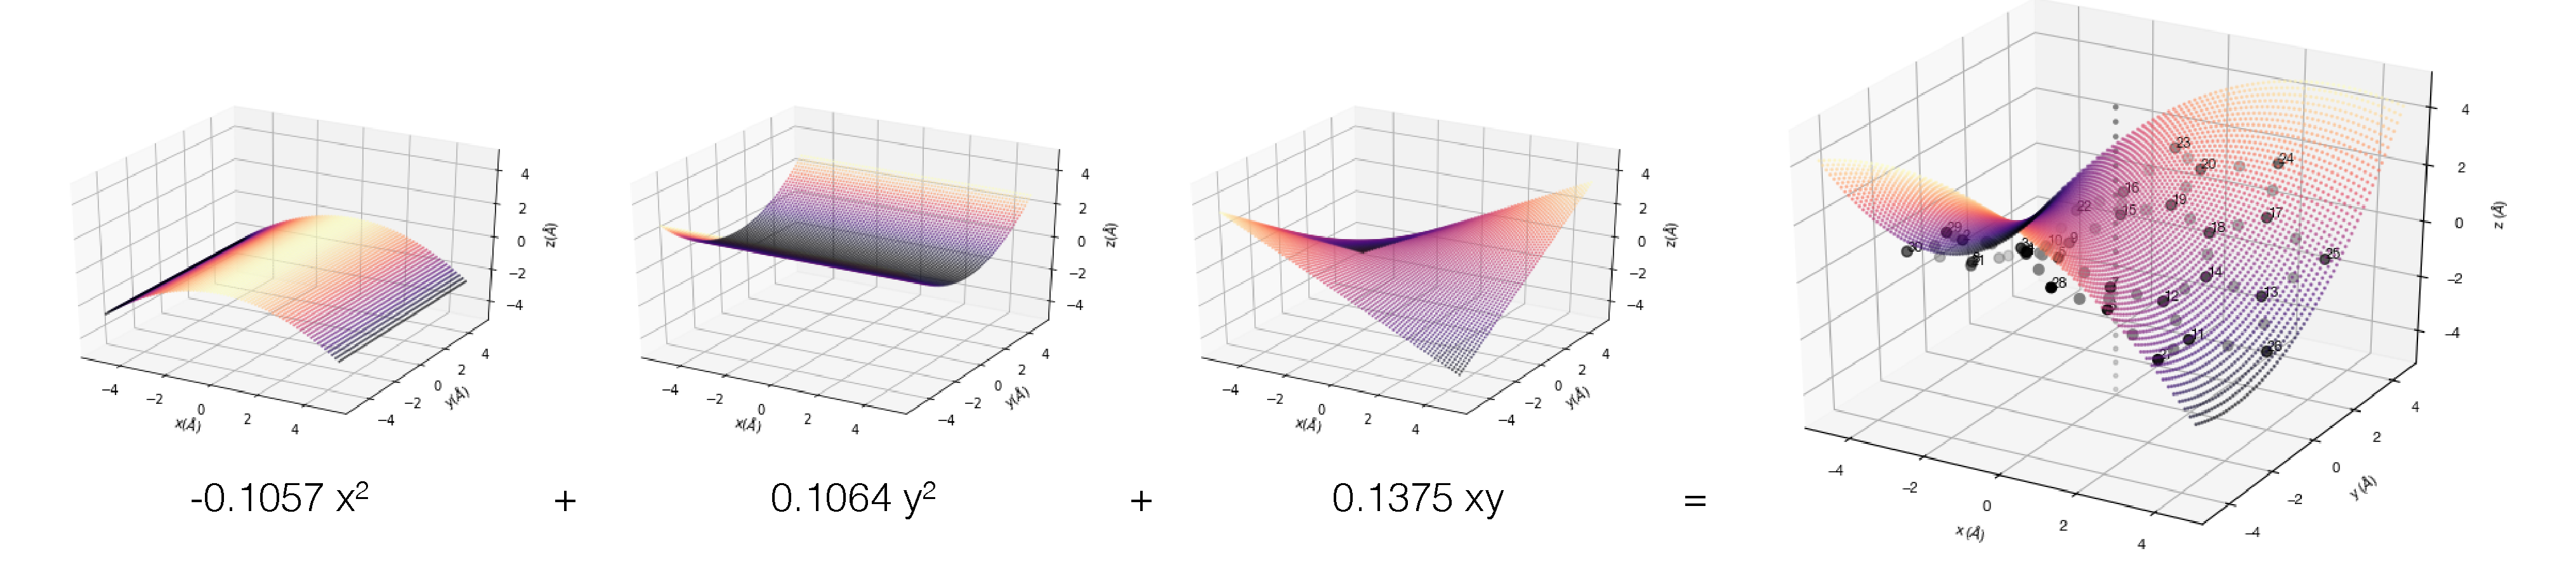
\includegraphics{linear-combination}
    \caption[Linear combination of base 3D functions]{Linear combination of base 3D functions to model the surface of Se10}
    \labfig{linear-combination}
\end{figure*}

After the surface has been defined, the results of the fitting are used to calculate a square grid of equally spaced points that are all equidistant to this molecule's surface.
In this case, a distance of \SI{1}{\angstrom} is set by general agreement with the literature.
Then, both the molecule atoms and the grid points are written into a Gaussian input file (the latter as dummy atoms), where the values of NICS will be calculated.
The calculation, specifically, estimates the values of the magnetic shielding using the Gauge-Independent Atomic Orbital (GIAO)\sidecite{keith93} method.

When the calculation is finished, the results can be visualized in 3D and plotted using the same program.
As it was previously said, through this technique aromatic compounds will experience shielding -negative values, marked in blue- on the inside of the ring and deshielding -positive values, marked in red- on the outside.
On the other hand, antiaromatic systems will experience the opposite effect.
This is the expected behavior and should be the basis for the evaluation of the technique, so to further verify it and illustrate it, the method has been applied to the well known model systems of benzene and cyclobutadiene.
Their 2D NICS graphs are included in \reffig{method-test}.

\begin{figure}[h]
    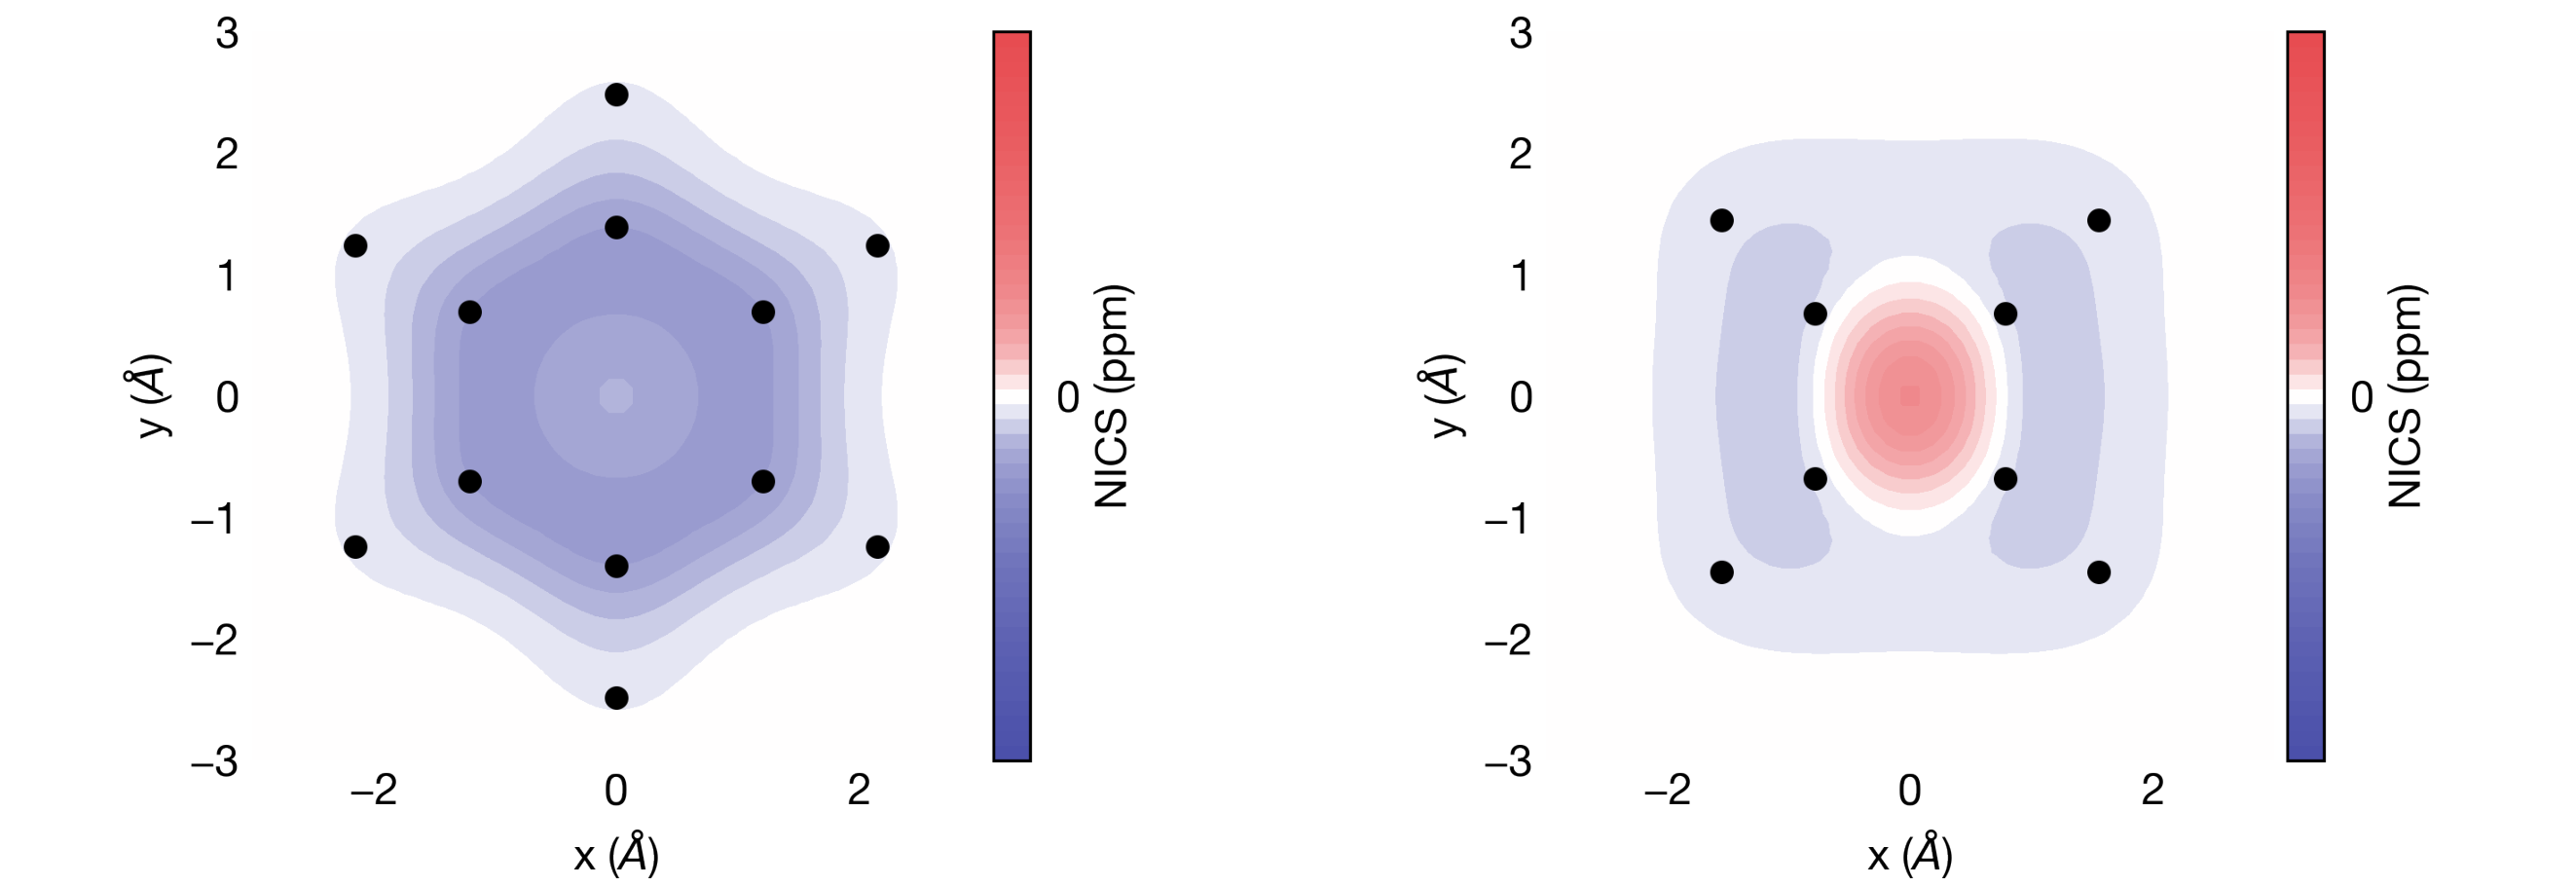
\includegraphics{method-test}
    \caption[NICS applied to test systems]{The custom NICS method, applied to benzene and cyclobutadiene from left to right}
    \labfig{method-test}
\end{figure}

The outcome for the Se10 calculation, plotted as a 2D projection onto the $xy$ plane, is displayed in \reffig{se10-2d}.
As it can be noted, all of the thiophene-like rings that comprise the structure seem to have negative values of NICS, while only in the very center of the whole flower there seems to be a tendency towards positive values.
This hints that the Se10 flower may have aromatic characteristics from a magnetic point of view.%
\begin{marginfigure}
    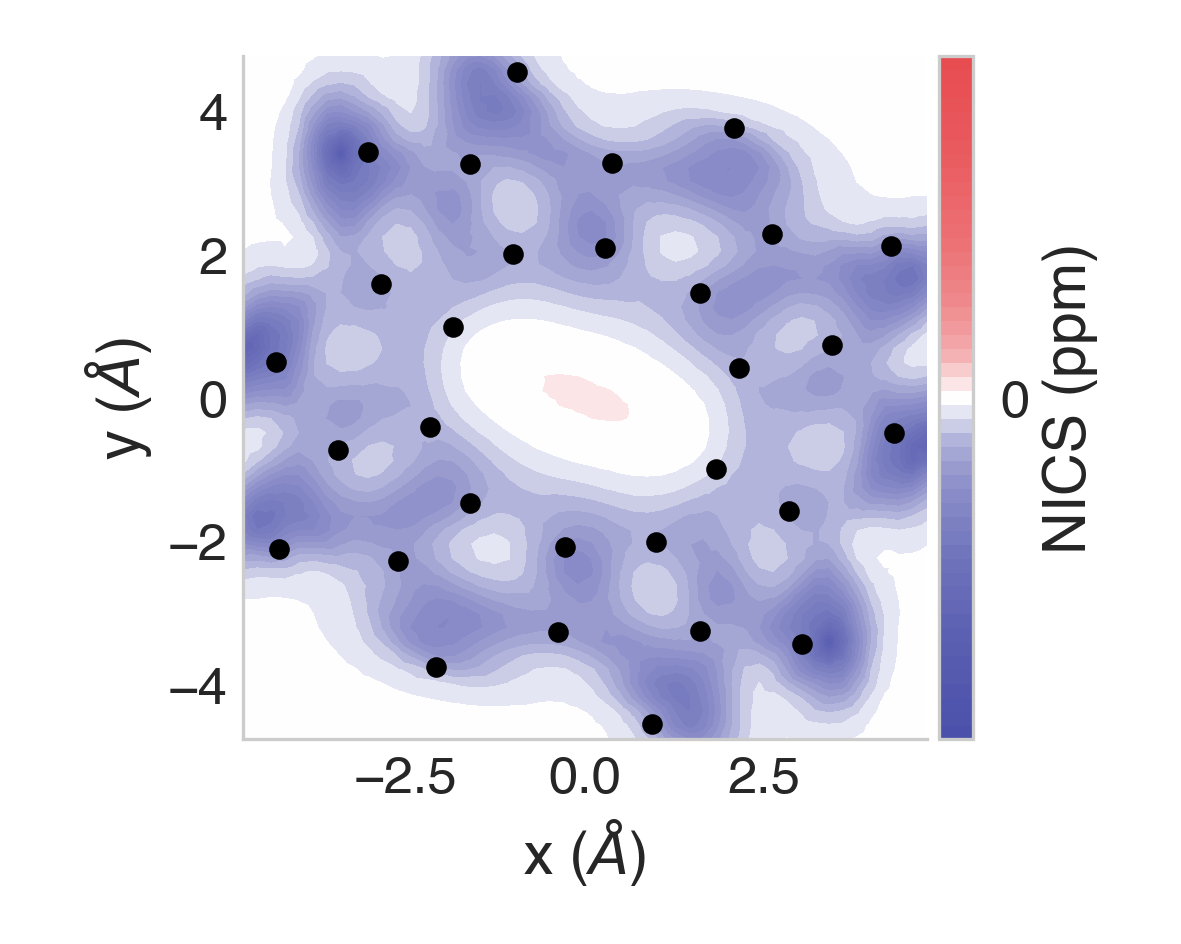
\includegraphics{se10-2d}
    \caption[NICS applied to Se10]{Custom NICS technique applied to the Se10 system}
    \labfig{se10-2d}
\end{marginfigure}%
Complementing this insight with the geometry metrics summarized in \reftab{bond-length-study}, which indicated that all of the bonds of the same type had approximately the same distances, we could say that Se10 has an aromatic character.

\blindtext

\begin{marginfigure}
    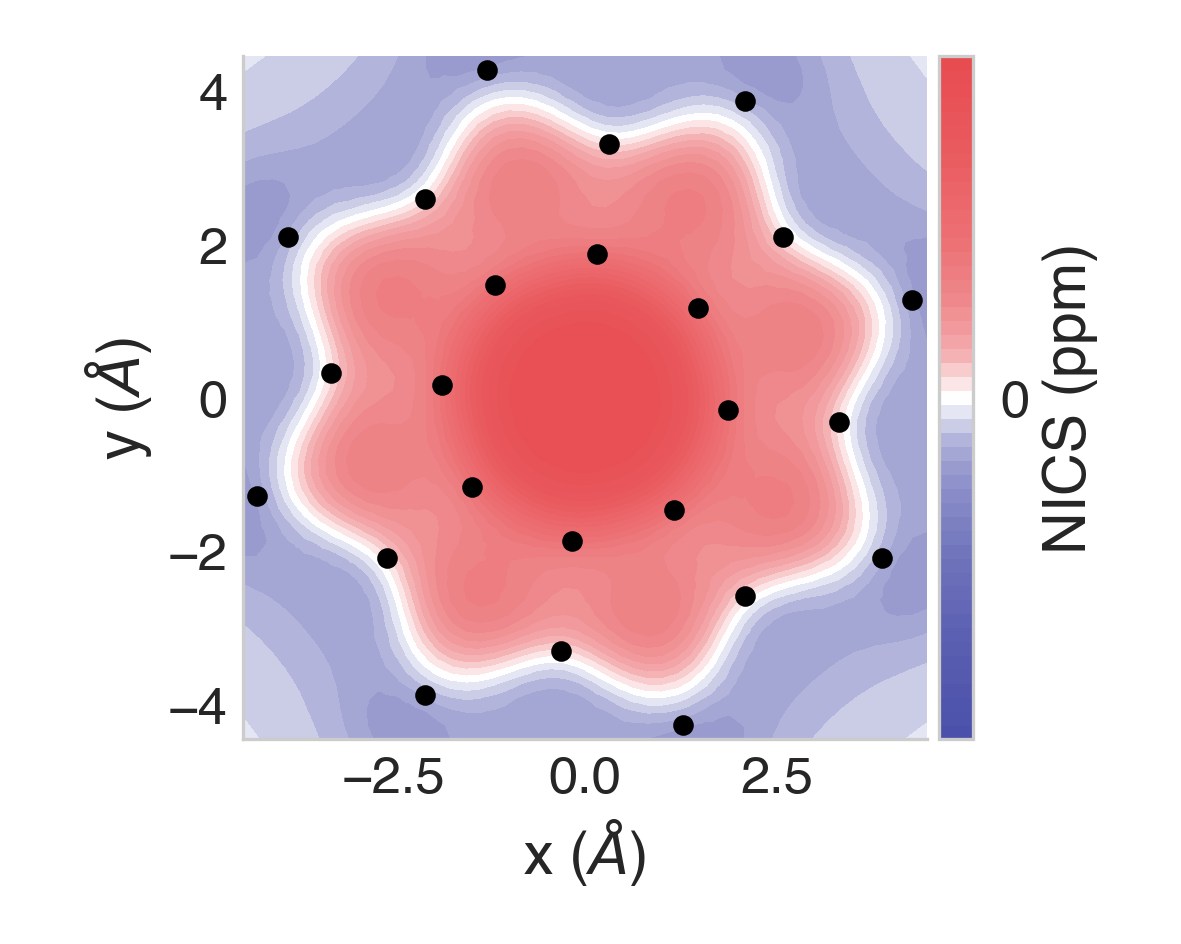
\includegraphics{as08-2d}
    \caption[NICS applied to As08]{Custom NICS technique applied to the As08 system}
    \labfig{as08-2d}
\end{marginfigure}

On the other hand, let's take the example of the As08 molecule.
Its NICS projection, plotted in \reffig{as08-2d}, shows positive values all through the inside of all of the rings, with negative values on the outside of the whole structure.
This behavior is much more similar to that of cyclobutadiene than to that of benzene as shown in \reffig{method-test}.
These magnetic properties, in addition to the fact that the lengths of its bond groups had noticeably higher standard deviations, hint towards an antiaromatic character.


\section{Spectroscopic characterization}
After having obtained a general profile of the nature of this novel family of molecules, we start delving into the main topic of the work: spectroscopy.

\subsection{Vibrational spectroscopy}
\labsec{raman-flowers}
Sunflowers of 8, 10 and 12 petals have 66, 84 and 102 vibrational modes, respectively.\marginnote{Any non linear molecule with $N$ atoms has $3N-6$ vibrational normal modes}
Depending on whether these vibrations actively affect the dipole or the polarizability of the flowers, they can be detected using infrared spectroscopy, Raman spectroscopy, or both.
In this work we will focus on the vibrational modes that are visible through Raman spectroscopy, as previously discussed in \refsec{previous-work}.

\subsubsection{Raman spectra}
Raman spectra for all 18 sunflower systems were generated following the procedures detailed in \refsec{spectra-envelope-calculation}.

Their vibrational profiles were quite simple, but quite varied.
However, one specially characteristic vibrational mode was found common to all of them: the symmetric and simultaneous stretching ($\nu_\textit{s}$) of all of the middle bonds (those formed between X$_0$ and X$_2$ atoms).
These special vibrations, referred to as \q{A} modes from now on, are associated to clean high intensity peaks in the spectrum, and are therefore easily identifiable.
In all of the generated Raman spectra, the A mode has been plotted as a vertical dashed line.
Other vibrational modes that were also deemed important were plotted using vertical solid lines.
These other modes, while still characteristic and useful for the identification of the flowers, were not as clean or easily describable as A modes.
They involved mixtures of asymmetric scissoring ($\delta_\textit{as}$) of the inner (X$_0$-X$_0$) and outer (X$_1$-X$_2$) bonds, and the asymmetric stretching ($\nu_\textit{as}$) of inner and middle bonds.

Using the Raman spectra of some of the 8 petal flowers as an example, plotted in \ref{fig:flower-raman}, it can be observed that they always have present an A-type mode at fairly similar frequencies.

\begin{figure*}[h]
    \label{fig:flower-raman}
    \centering
    \begin{subfigure}{8.25cm}\centering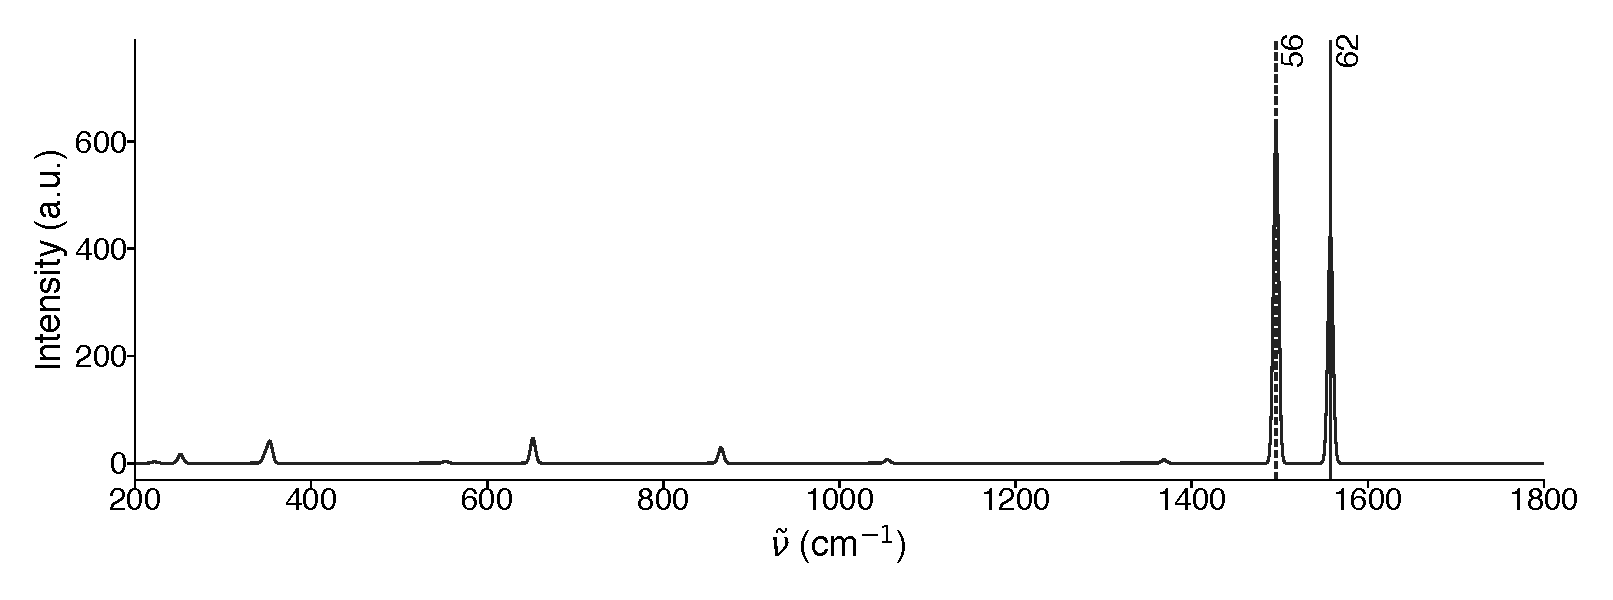
\includegraphics{raman-s08}\caption{Raman spectrum for S08}\end{subfigure}%
    \begin{subfigure}{8.25cm}\centering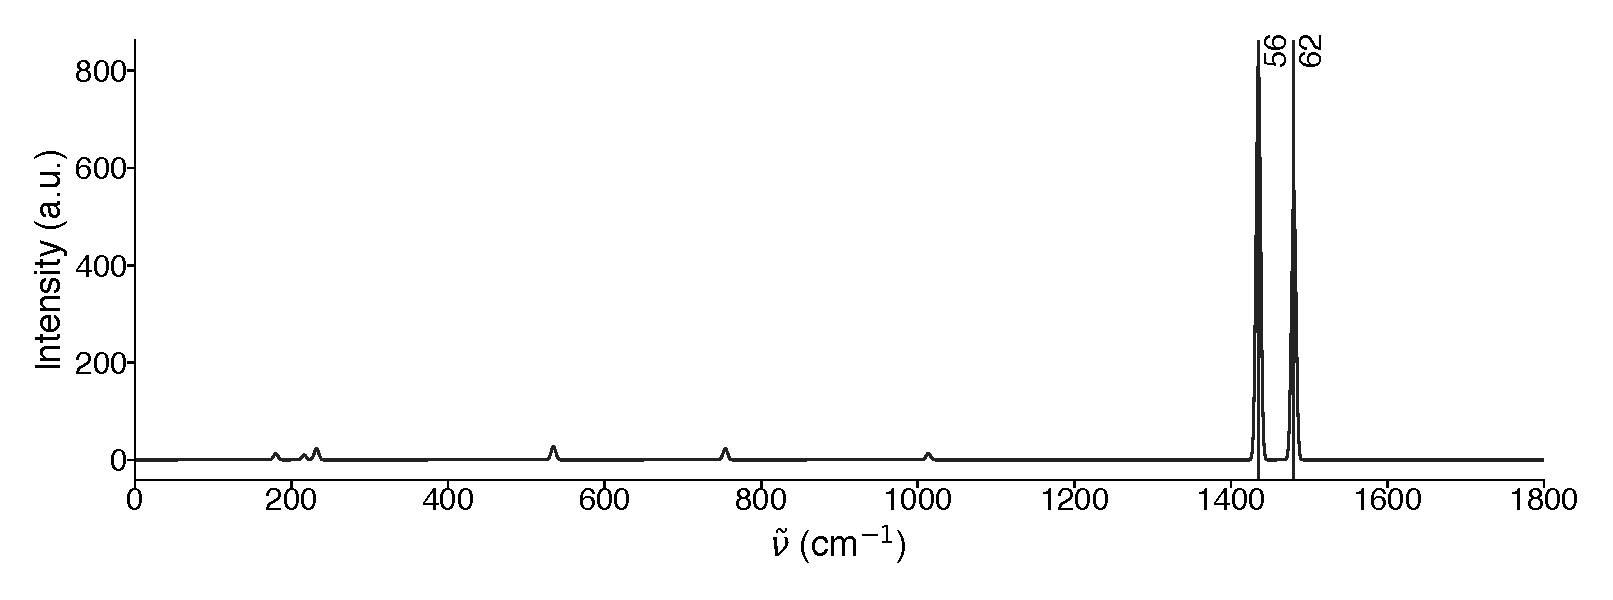
\includegraphics{raman-se08}\caption{Raman spectrum for Se08}\end{subfigure}
    \begin{subfigure}{8.25cm}\centering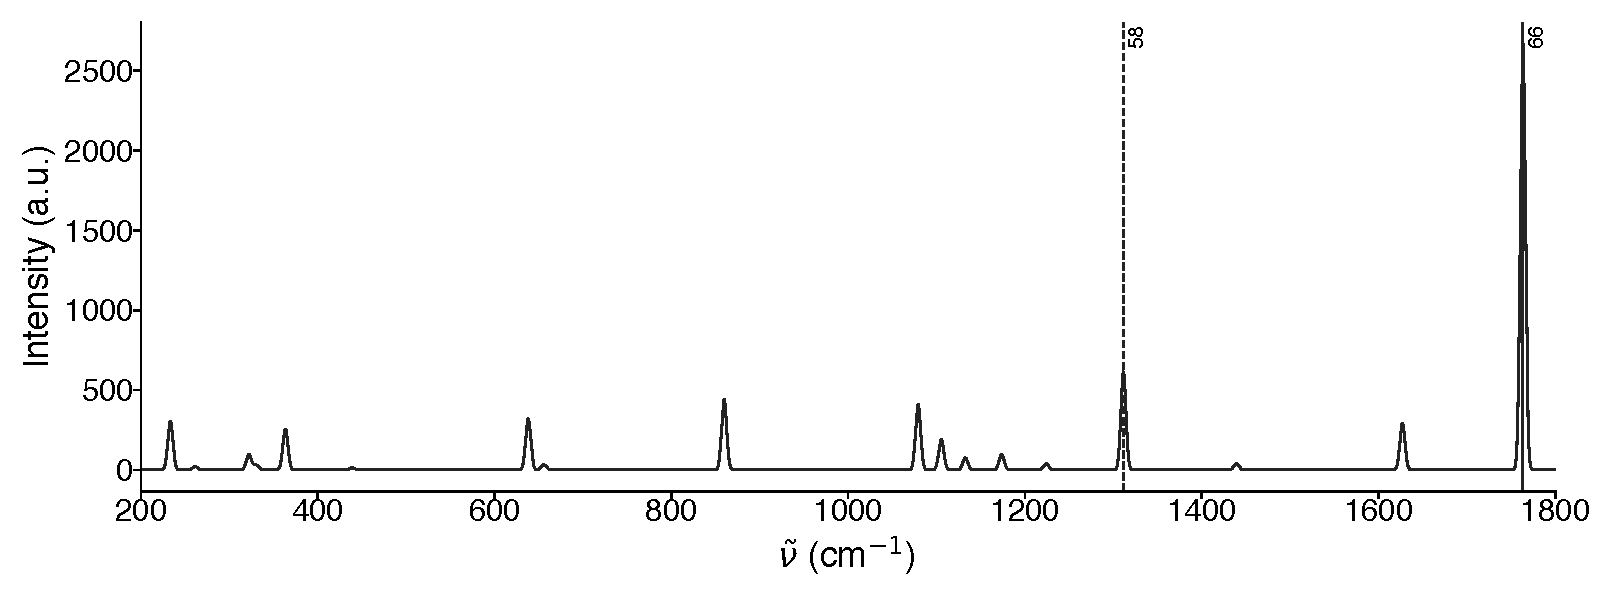
\includegraphics{raman-p08}\caption{Raman spectrum for P08}\end{subfigure}%
    \begin{subfigure}{8.25cm}\centering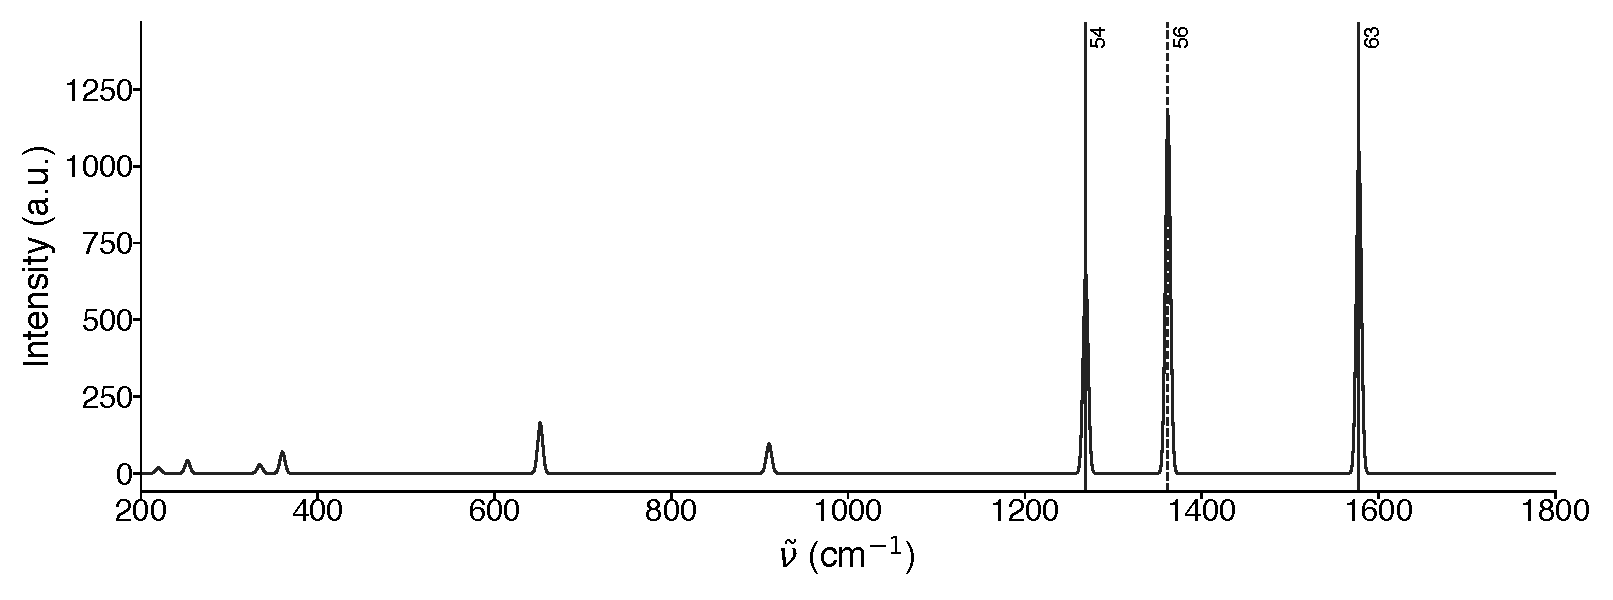
\includegraphics{raman-pn08}\caption{Raman spectrum for PN08}\end{subfigure}
    \caption[Raman spectra of 8 petal flowers]{Raman spectra of a selection of 8 petal flowers. Note the A modes plotted with dashed lines}
\end{figure*}

Additionally, in general, an increase in the complexity of the spectra and a decrease in the cleanliness of the spectra was observed alongside the increase of the number of petals: flowers with 12 petals had more complex patterns of modes than flowers with 8.

Let's take, for example, the As family.
The spectra for As08 and As12, displayed  in \ref{fig:as-raman}, have clear differences in intricacy and number of modes.

\begin{figure*}[h]
    \label{fig:as-raman}
    \centering
    \begin{subfigure}{8.25cm}\centering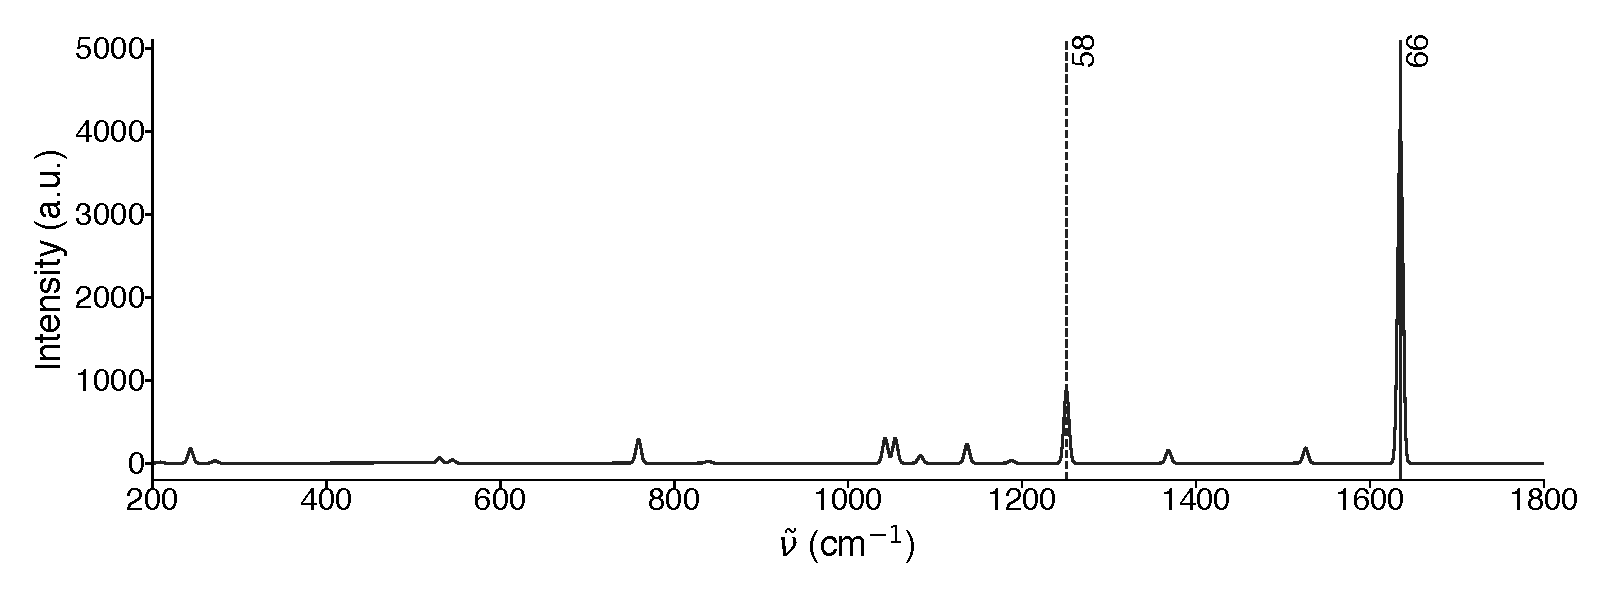
\includegraphics{raman-as08}\caption{Raman spectrum for As08}\end{subfigure}%
    \begin{subfigure}{8.25cm}\centering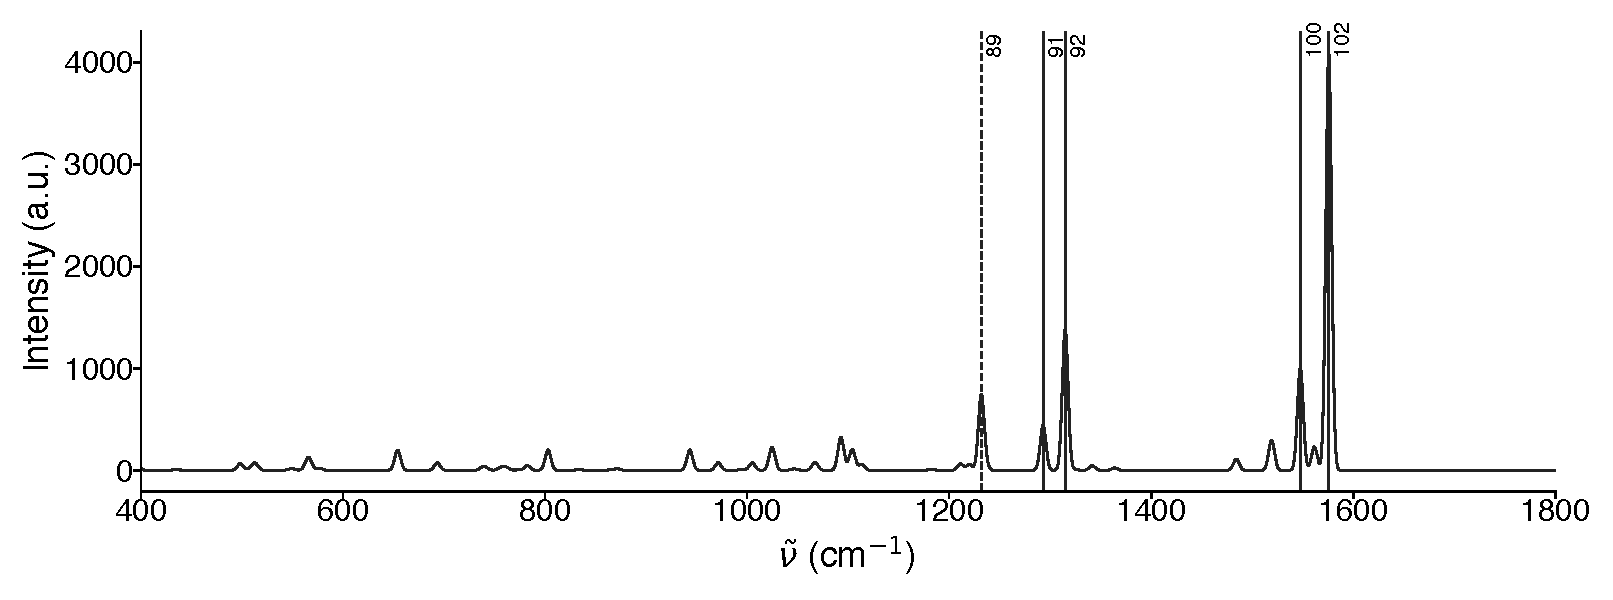
\includegraphics{raman-as12}\caption{Raman spectrum for As12}\end{subfigure}
    \caption[Raman spectra of As08 and As12]{Raman spectra of As08 and As12}
\end{figure*}

All in all, these spectra were considered simple and clear enough to allow for the identification of the flowers.
The other spectra that weren't displayed in this section can be found in \refsec{ap:raman-flowers}.

\subsection{Electronic spectroscopy}
\labsec{uv-sunflowers}
Keeping in mind the final objectives of the work of applying resonance Raman, the electronic spectroscopic behavior of the flowers was deemed as a relevant point to study: the characterization of the electronic transitions of a molecule might yield insight about its interactions with light.

\subsubsection{UV-vis spectra}
The most straightforward way to study electronic spectroscopy is by simulating ultraviolet-visible (UV-vis) spectra.
In order to generate this, the energies of the 50 first transitions from the ground state to excited states were computed using TD-DFT in the Gaussian09 suite.
Then, using their energy and oscillator strength values, Gaussian functions were calculated for each of the transitions and linearly combined to create continuous spectra similar to those obtained using real spectrophotometers.
This procedure is further explained in \refsec{spectra-envelope-calculation}.
UV-vis spectra were generated for all of the sunflowers, but since they are fairly simple graphs, only the one for S08 will be explained in this section as an example.
It's displayed in \reffig{uv-s08-simple}.

\begin{figure}[h]
    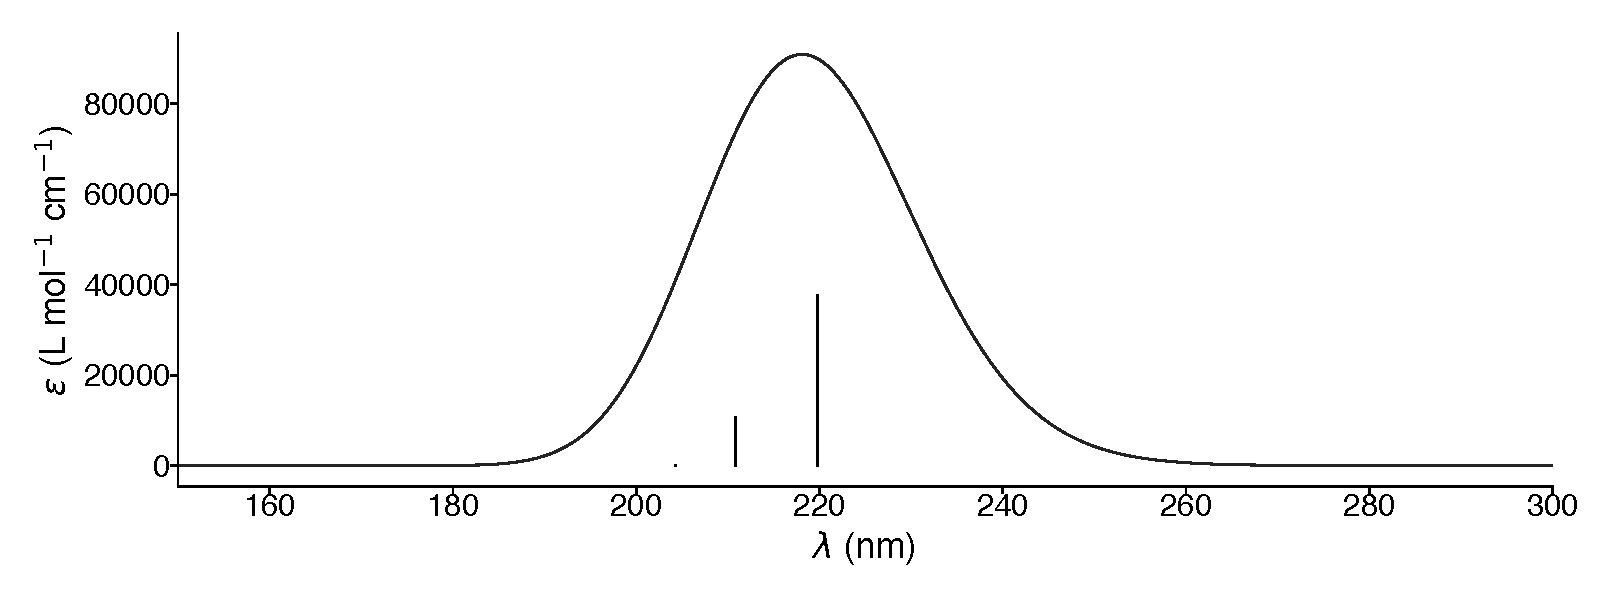
\includegraphics{uv-s08-simple}
    \caption[UV-vis spectrum of S08]{UV-vis spectrum of S08}
    \labfig{uv-s08-simple}
\end{figure}

\begin{margintable}
    \centering
    \caption[UV-vis absorption range of isolated flowers]{Approximate UV-vis absorption range of isolated flowers}
    \begin{tabular}{@{}rc@{}}
        \toprule
        System & $\lambda$ (\si{\nano\metre}) \\
        \midrule
        S08 & 180-260 \\
        S10 & 180-280 \\
        S12 & 200-400 \\
        Se08 & 200-280 \\
        Se10 & 200-400 \\
        Se12 & 225-500 \\
        As08 & 250-800 \\
        As10 & 250-700 \\
        As12 & 300-900 \\
        AsN08 & 300-450 \\
        AsN10 & 300-650 \\
        AsN12 & 300-850 \\
        P08 & 225-700 \\
        P10 & 250-500 \\
        P12 & 250-700 \\
        PN08 & 250-500 \\
        PN10 & 250-550 \\
        PN12 & 300-700 \\
    \end{tabular}
    \labtab{flower-uv-ranges}
\end{margintable}

We can see that the spectrum for S08 goes from \SI{190}{\nano\metre} to \SI{260}{\nano\metre}, approximately.
Plotted as straight vertical lines, the individual electronic transitions have been included, where their height is proportional to their oscillator strength.
However, this is not an adequate representation in this case.
What appear to be 2 electronic transitions located at \SI{210}{\nano\metre} and \SI{219}{\nano\metre} are, in fact, 4 different transitions (specifically, there are 2 groups of 2 each): it's just that due to the high symmetry of the molecule, transitions that occur in regions of the molecule that are very electronically similar might have coinciding wavelengths.

This was true for most of the flowers: many of the transitions with the higher intensities were grouped in pairs.
The only cases where this effect didn't clearly happen were the sunflowers with the most warped and most bent geometries, such as As12, AsN12, P12 and PN12.

In any case, since the purpose of studying individual electronic transitions is to serve as a guide when applying resonance techniques and we won't study the resonance of the isolated flowers, they were left out of the spectra.

The rest of the UV-vis spectra of the flowers may be found in \refsec{ap:uv-vis-flowers}.
Their absorption ranges, nonetheless, have been summarized and presented in \reftab{flower-uv-ranges} as an overview.

\section{Conclusions}

Summarizing this whole chapter into a list of important points:

\begin{itemize}
    \item The family of molecules of the study, collectively named as \q{flowers} or \q{sunflowers}, was built using molecules based on \q{sulflower} using S, Se, As, As+N, P and P+N as substituents
    \item Flowers with 8, 10 and 12 petals were generated due to their higher structural and electronic stability, resulting in a total of 18 different molecules
    \item Statistical analysis was performed on the length of their bonds, and the values of their mean and standard deviation were considered as early indicatives of their stability and their possible conjugation effects
    \item The strain energy for each flower was calculated through the design of a homodesmotic reaction
    \item Aromaticity was directly studied using an approach designed and programmed by the author using multiple linear regression and NICS. It was found that all flower groups except for As and P exhibited magnetic behavior that hinted towards aromatic character
    \item The Raman active vibrational modes of the flowers were briefly characterized and plotted as Raman spectra
    \item The electronic spectroscopy of the flowers was studied by generating their UV-vis spectra
\end{itemize}

All in all, all of the studied flowers were considered stable and interesting enough to be applied to the STX problem as surface-like adsorption substrates.
